\chapter{自动化与引用}

% =========================================================
\section{交叉引用：Label 与 Ref 的自动编号}

% --- 讲解部分 ---
\LaTeX{} 的自动化核心在于“标签-引用”机制。通过给图表、公式或章节定义一个唯一的标签（\texttt{\textbackslash label}），你可以在正文任何地方调用它的编号 。
无论你后期如何增删内容，\LaTeX{} 都会在编译时自动重新计算所有编号，确保引用永不失效 。

% --- 演示部分 ---
\begin{figure}[H]
	\centering
	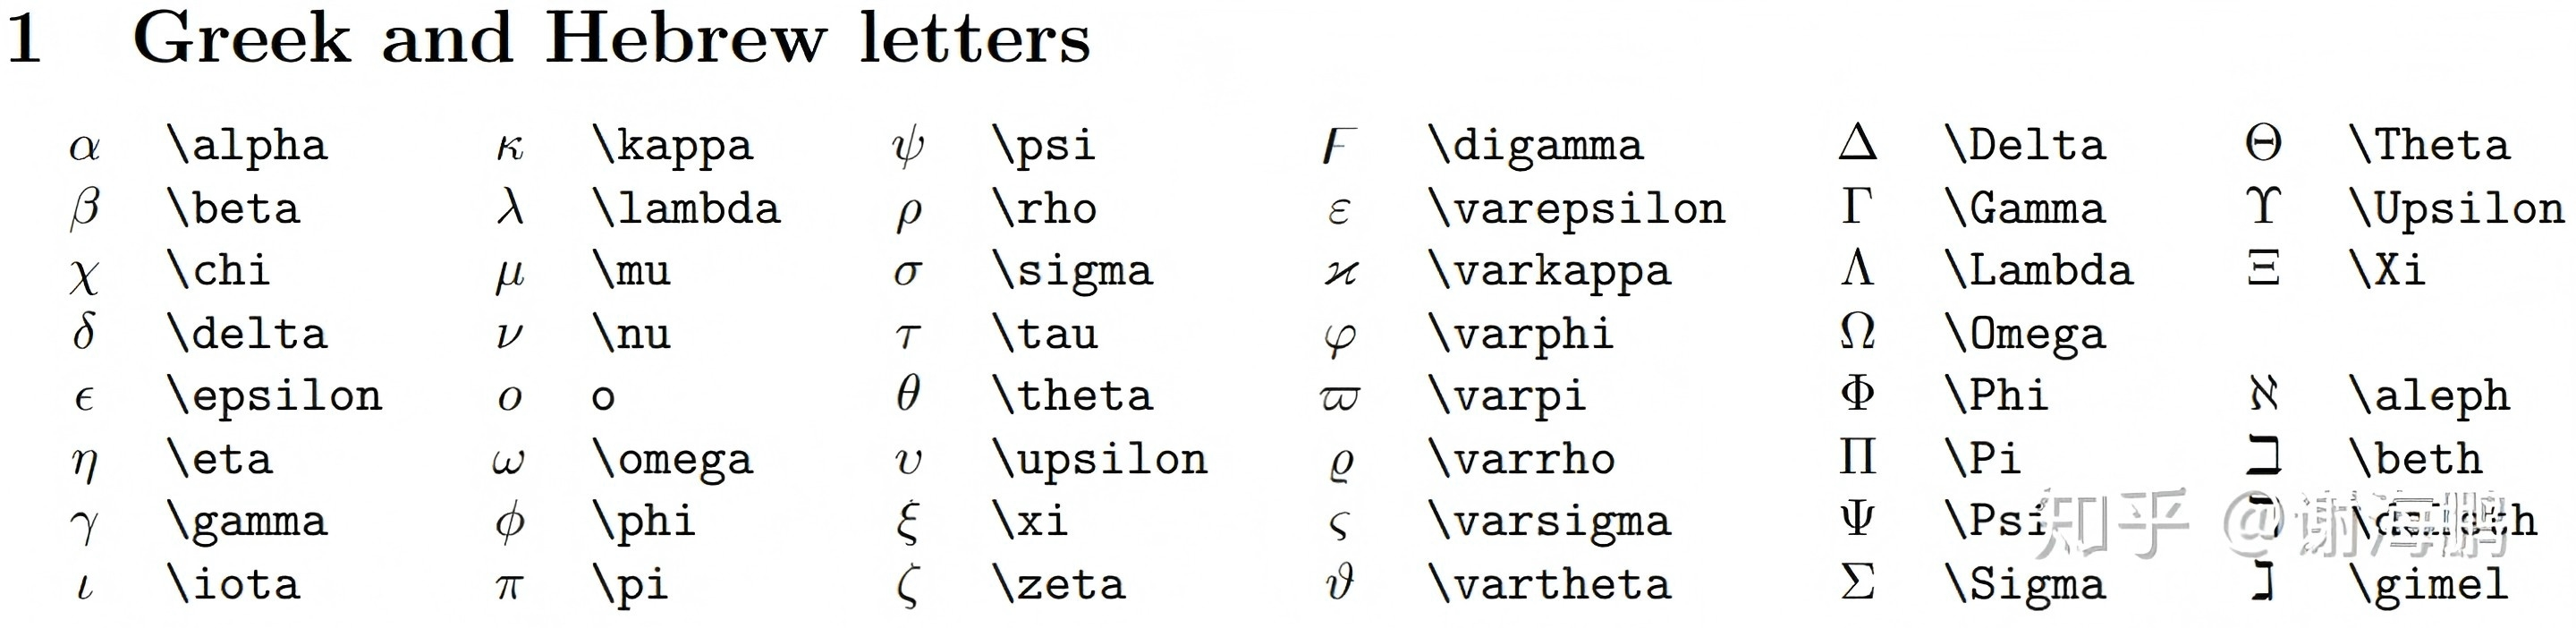
\includegraphics[width=0.4\textwidth]{Figure/1.jpg}
	\caption{系统架构示意图}
	\label{fig:system_arch} % 定义标签
\end{figure}

如或图 \ref{fig:system_arch}所示，该架构展示了系统的核心组成部分。

\begin{equation}
	E = mc^2 \label{eq:energy}
\end{equation}

质能方程（见公式 \ref{eq:energy}）揭示了质量与能量的等价性。

% =========================================================
\section{参考文献：BibTeX 数据库与引用样式}

% --- 讲解部分 ---
管理参考文献最专业的方式是使用 BibTeX 。
1. \textbf{创建数据库}：新建一个 \texttt{.bib} 文件（如 \texttt{refs.bib}），存入文献条目 。
2. \textbf{正文引用}：使用 \texttt{\textbackslash cite\{key\}} 命令 。
3. \textbf{生成列表}：在文档末尾指定样式并导入数据库 。

% --- 演示部分 ---
\begin{lstlisting}[language={[LaTeX]TeX}, caption={BibTeX 数据库条目示例}]
	@article{Einstein1905,
		author  = "Albert Einstein",
		title   = "Does the Inertia of a Body Depend upon Its Energy-Content?",
		journal = "Annalen der Physik",
		year    = "1905"
	}
\end{lstlisting}

引用演示：根据爱因斯坦的研究 \cite{Einstein1905}，我们可知能量的变化会导致质量的变化。

% =========================================================
\section{自动生成目录与索引}

% --- 讲解部分 ---
只要正确使用了 \texttt{\textbackslash chapter} 和 \texttt{\textbackslash section} 等命令，\LaTeX{} 就能自动提取标题并生成带页码的目录 。

\begin{itemize}
	\item \texttt{\textbackslash tableofcontents}：生成章节目录 。
	\item \texttt{\textbackslash listoffigures}：生成图片清单 。
	\item \texttt{\textbackslash listoftables}：生成表格清单 。
\end{itemize}

\begin{tcolorbox}[colback=red!5, colframe=red!50, title=使用技巧]
	由于 \LaTeX{} 需要先扫描标签再填入编号，涉及交叉引用和目录时，通常需要\textbf{编译两次}才能完全显示正确结果 。
\end{tcolorbox}

这个部分你要用的话可以单独学？maybe我到时候教你？hhh